% Created 2020-09-16 Wed 04:40
% Intended LaTeX compiler: lualatex
\documentclass[11pt]{article}
\usepackage{graphicx}
\usepackage{grffile}
\usepackage{longtable}
\usepackage{wrapfig}
\usepackage{rotating}
\usepackage[normalem]{ulem}
\usepackage{amsmath}
\usepackage{textcomp}
\usepackage{amssymb}
\usepackage{capt-of}
\usepackage{hyperref}
\usepackage{tabularx}
\usepackage{etoolbox}
\makeatletter
\def\dontdofcolorbox{\renewcommand\fcolorbox[4][]{##4}}
\AtBeginEnvironment{minted}{\dontdofcolorbox}
\makeatother
\usepackage[newfloat]{minted}
\author{Mark Armstrong}
\date{\today}
\title{The Boom hierarchy in Scala}
\hypersetup{
   pdfauthor={Mark Armstrong},
   pdftitle={The Boom hierarchy in Scala},
   pdfkeywords={},
   pdfsubject={A brief background on the Boom hierarchy family of datatypes, followed by a (in the end, flawed) implementation in Scala.},
   pdfcreator={Emacs 27.0.90 (Org mode 9.3.8)},
   pdflang={English},
   colorlinks,
   linkcolor=blue,
   citecolor=blue,
   urlcolor=blue
   }
\begin{document}

\maketitle
\tableofcontents


\section{Introduction}
\label{sec:orga78652b}
These notes were created for, and in some parts \textbf{during},
the lecture on September 14th and the following tutorials.

\section{Motivation}
\label{sec:org14e8c25}

\subsection{Scala as an object-oriented language}
\label{sec:orgc3cfb30}

Scala is a purely-object oriented language,
meaning that every value is an object (contrast this
with languages such as Java where some values
are “basic” and not objects).

Scala interops with Java, meaning that Java libraries can be used
in Scala code. It also supports many Java abstractions/constructs,
so it can be a (fairly) comfortable transition for Java programmers.

For instance, if we want to define a linked list type in Scala,
we can take an approach similar to what we might do in Java.
(This is a very naive definition and usage,
but it serves to prove the point.)
\begin{minted}[breaklines=true]{scala}
// Type annotations come after names, and are separated by a `:`.
// The `var` keyword indicates a variable.
class LinkedList[A](var hd: A, var tl: LinkedList[A]) {

  // Methods/functions are type annotated like values.
  // Scala uses an `=` in method/function declarations.
  // to emphasise that they should return a value.
  def head: A = {
    hd   // No semicolons necessary; a newline will do.
  }

  // No braces are needed if the right side's a single expression.
  def tail: LinkedList[A] = tl
}

// `val`'s are constant, unlike `var`'s.
val l1: LinkedList[Int] = new LinkedList[Int](1, null)

// There's no need to specify a type if Scala can infer it.
// Here it can see that the type parameter `A` is `Int` on the right.
val l2: LinkedList[Int] = new LinkedList(2, l1)

// In fact, it can tell the type of the `val` too.
val l3 = new LinkedList(3, l2)


// Let's define a value as a quick sanity test.
val test1 = l1.head == 1
\end{minted}

But this is only one part of Scala,
and for our purposes it's the less interesting part.
(We could just use Java for this much.)

\subsection{Scala as a functional language}
\label{sec:orgdf45b44}

We are interested in Scala primarily because it supports
functional abstractions.

The distinguishing abstractions of
functional programming languages are:
\begin{enumerate}
\item Functions are values, i.e., data.
\begin{itemize}
\item This is referred to by the term “first-class functions”,
implying that functions are not excluded
from being treated as data.
\item This allows for \emph{higher-order} functions;
functions which take other functions as argument.
\end{itemize}
\item All values (data) are \emph{immutable}.
\begin{itemize}
\item (At least in “pure” functional languages.)
\item Variables still change throughout the program,
but only because they are bound to different values
at different points in the runtime.
Not because an assignment/update was carried out.
\begin{itemize}
\item For instance, in a recursive call, the arguments change.
\end{itemize}
\end{itemize}
\end{enumerate}

We will concern ourselves with (1) another time.
For today, we are considering (2).

Briefly, the advantage to immutable data is that
enables the programmer a level of certainty that is not available
if data is mutable.

Consider for a moment this pseudocode regarding our earlier linked lists.
\begin{verbatim}
// This is pseudocode
val l1: LinkedList[Int] = null

somebodyElsesFunction(l1)
\end{verbatim}
What can I say about my list \texttt{l1} after I run “somebody else's”
function on it?

:TODO:

\subsubsection{Aside: Downside to immutability}
\label{sec:org456ed64}

There is a not insignificant downside to enforcing immutability
in a language/code base.

If all data is immutable, then to “make changes” to a value
(such as a list or a tree),
we must in fact make a copy of that value
with the changes we want applied.

As you can imagine, this copying is expensive,
both in terms of space and time.

\emph{However}, well-designed languages can mitigate this
in various ways, including by having values “share”
some pieces of themselves.

\section{The (extended) Boom hierarchy\hfill{}\textsc{theory}}
\label{sec:orged9e269}
We now briefly take with a (relatively brief) dive into some theory,
to give us an example type to consider in Scala.

\subsection{Introduction}
\label{sec:org56f8a0c}
The Boom hierarchy was introduced
by \href{https://www.kestrel.edu/people/meertens/publications/}{Lambert Meertens} in
\href{https://www.kestrel.edu/people/meertens/publications/papers/Algorithmics.pdf}{Algorithmics — Towards programming as a mathematical activity};
Meertens attributes the concept to H. J. Boom, hence the name.

The Boom hierachy is a family of data structures
—namely trees, lists, bags and sets—
for which we have an \texttt{empty} value and can construct \texttt{singleton} values,
and which include a \texttt{join} operation
(for sets and bags also called \texttt{union}, written \texttt{∪},
and for lists also called \texttt{append}, \texttt{++}).

:TODO:
Notation:
\begin{itemize}
\item \texttt{[]} for empty,
\item \texttt{[a]} for a singleton containing \texttt{a},
\item \texttt{++} for append.
\end{itemize}

The basic idea of the hierarchy is that
\begin{itemize}
\item sets have a \texttt{join} operation which
\begin{itemize}
\item has an identity \texttt{A ∪ ∅ = A},
\item is idempotent \texttt{A ∪ A = A},
\item is commutative \texttt{A ∪ B = B ∪ A}, and
\item is associative \texttt{A ∪ (B ∪ C) = (A ∪ B) ∪ C}. Then,
\end{itemize}
\item bags are like sets, except the \texttt{join} operation is not idempotent,
\item lists are like bags, except the \texttt{join} operation is not commutative, and
\item trees are like lists, except the \texttt{join} operation is not associative.
\end{itemize}

The paper is interested in laws satisfied by the
higher-order functions \texttt{reduce} (often called \texttt{fold}),
\texttt{map} and \texttt{filter} over those structures.

\subsection{Extending the Boom hierarchy}
\label{sec:org40b4064}
Alexander Bunkenburg's later paper
“\href{https://citeseerx.ist.psu.edu/viewdoc/download?doi=10.1.1.49.3252\&rep=rep1\&type=pdf}{The Boom Hierarchy}” 
investigates this area further, by considering
what data structures can be obtained by taking different combinations
of the above listed features of the \texttt{join} operation.
The abstract of that paper reads
\begin{quote}
“The Boom Hierarchy is the family of data structures tree, list, bag, set.
By combining their properties in other ways,
more data structures can be made, like mobiles.
The paper defines the data structures of this extended Boom Hierarchy
and shows how the functions reduce, map, and filter are applied to them.”
\end{quote}

For instance, through this process we arrive at
\begin{itemize}
\item the \texttt{nonempty list} data structure or \texttt{nonempty tree} data structure,
which lack an identity.
\item the \texttt{mobile} data structure, which are like trees
except that they “can spin” (the branching order is arbitrary).
\end{itemize}

\subsection{Visualising the Boom hierarchy}
\label{sec:org8d3a974}
We can visualise the layout of some of these structures:
\begin{center}
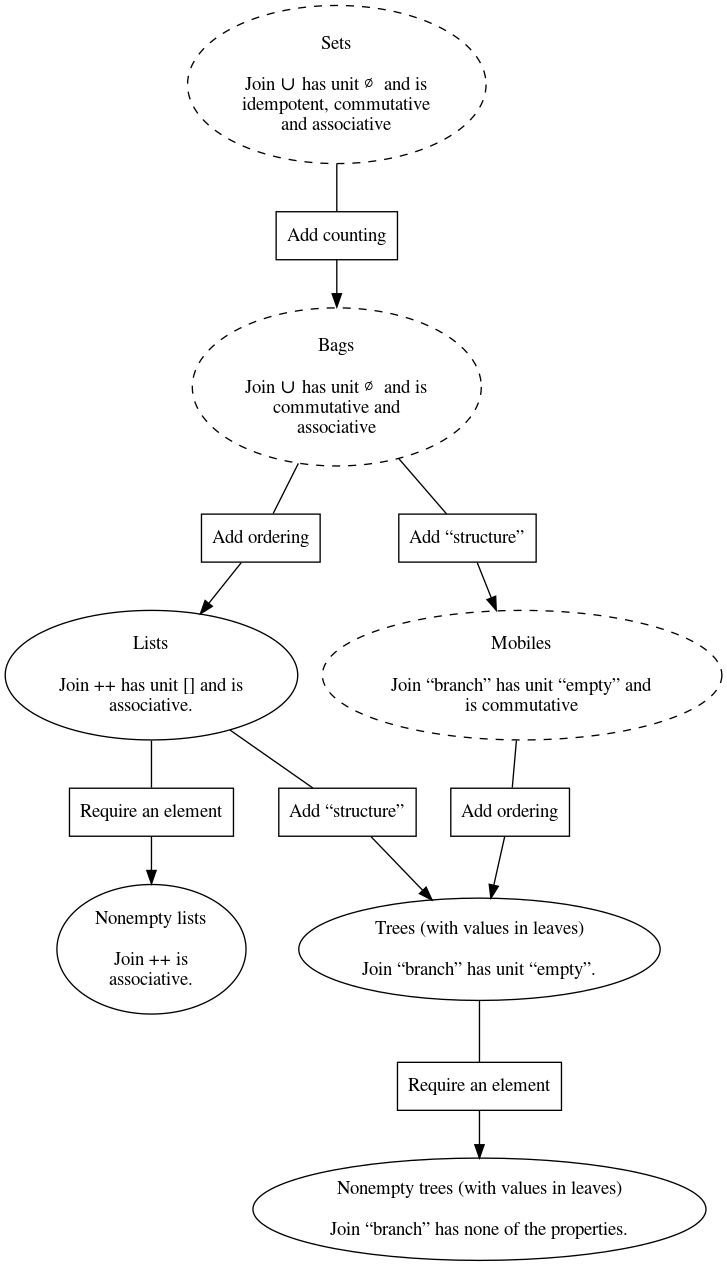
\includegraphics[width=\textwidth]{media/BOOM.png}
\end{center}

Not all of these types are easily representable in most programming languages;
we can say they are \emph{abstract} types instead of \emph{concrete} types.
I've highlighted the ones which are not in the diagram using dashed lines.

Exercise: Why are those types not easily represented in standard
programming languages?

Exercise: Is it impossible for those types to be easily represented
in a programming language?

\section{The Boom hierarchy in Scala\hfill{}\textsc{application}}
\label{sec:orge3329ae}
\begin{center}
\textbf{Heads up: this section consists of failed attempts}
\textbf{and subsequent corrections. Read carefully, and double check}
\textbf{before borrowing any code. Or skip to the next section.}
\end{center}

Let us try to implement the lists discussed in the Boom hierarchy
in Scala, and make them \emph{immutable}, for the reasons discussed in
\hyperref[sec:orgdf45b44]{Scala as a functional langauge}.

\subsection{The \texttt{AppendList} type}
\label{sec:org251ed6a}
Let us implement the list type as described in the Boom hierarchy paper
in Scala. We'll call these \texttt{AppendList}, as they take \texttt{Append} as
the basic operation.

\begin{center}
\textbf{Extra heads up: there's a big flaw in defining lists this way,}
\textbf{so even when we get it right we're wrong.}
\textbf{We'll discuss the problem at the end.}
\end{center}

Those lists have three cases;
\begin{itemize}
\item the \texttt{Empty} list,
\item the \texttt{Single}-ton lists, and
\item the \texttt{Concat}-enation of two lists.
\end{itemize}

The Scala convention for implementing types such as this
that consist of a number of cases by first giving
a \emph{super-type} which a \emph{sub-type}
for each case will \emph{extend} (extending is also called inheriting).

This super-type should not be instatiable,
because we want to restrict instatiability to the given cases.
(Recall from 2fa3: types should have \textbf{no junk} and no confusion.) 

A \texttt{trait} is similar to a \texttt{class}, except it cannot be instantiated
—meaning it cannot be constructed.
It is similar to an \texttt{interface} in Java.
(This also makes it similar to an \texttt{abstract class},
except it's more flexible; see
\href{https://docs.scala-lang.org/overviews/scala-book/abstract-classes.html}{the Scala docs}.)
\begin{verbatim}
trait AppendList[A]
// sub-class definitions yet to come
\end{verbatim}

In fact, in the interest of not introducing “junk”,
we should use the \texttt{sealed} keyword which prevents code
from outside this block from extending \texttt{AppendList}.
\begin{verbatim}
sealed trait AppendList[A]
\end{verbatim}

\subsection{Attempt 1 at defining cases of lists: basic classes}
\label{sec:orgea12cf9}
Now we need to add sub-types which are instantiable.
Note that every instance (value) of one of the sub-types
is also a value of the super-type.
So even though \texttt{AppendList} cannot be instantiated,
we can create \texttt{AppendList} values.

(Yes, this means a single value can have many types;
specifically, it has a chain of types, each one a sub-type of the next).
:TODO: where does the chain end?

We can fill in a \texttt{class} for each case.
\begin{minted}[breaklines=true]{scala}
trait AppendList[A]
class Empty[A]() extends AppendList[A]
class Single[A](a: A) extends AppendList[A]
class Concat[A](l: AppendList[A], r: AppendList[A]) extends AppendList[A]
\end{minted}

But if we try out this definition, we may be disappointed.
\begin{minted}[breaklines=true]{scala}
val empty1 = new Empty[Int]
val empty2 = new Empty[Int]

val list1 = new Concat(new Single(1), new Single(2))

empty1 == empty2  // equality check
\end{minted}
:TODO: why? what's so bad about the result of the equality check?

\subsubsection{Aside: Notions of equality}
\label{sec:org5768a5e}

:TODO:

\subsection{Attempt 2 at defining cases of lists: case classes}
\label{sec:org72390be}
Our \texttt{class} based definition above caused two instances
of the same list (same in the sense that their construction was the same)
as different (unequal) lists.

The reason comes back to mutability.
A regular \texttt{class} may have mutable data (non-constant fields).
So the runtime is aware that \texttt{empty1} and \texttt{empty2} could
actually be different (even though, with just our definitions above,
there isn't a way to make them significantly different).

Since we intend to work with immutable data,
we need something more than just \texttt{class}.

Specifically, what we want is provided in
Scala by a \texttt{case class}.
A \texttt{case} class has no mutable state (no non-constant fields).
(Additionally all its fields are public).
\begin{minted}[breaklines=true]{scala}
sealed trait AppendList[A]
case class Empty[A]() extends AppendList[A]
case class Single[A](a: A) extends AppendList[A]
case class Concat[A](l: AppendList[A], r: AppendList[A]) extends AppendList[A]
\end{minted}

The name \texttt{case class} is used because
we often \emph{pattern match} (or, equivalently, \emph{case split})
over types defined this way.

\subsection{The inherent problem with \texttt{AppendList}}
\label{sec:org1bb0728}
\begin{quote}
“Each data structure is the free algebra of its binary operation \texttt{++.}”
\end{quote}

:TODO: \textbf{no confusion}!

\begin{minted}[breaklines=true]{scala}
sealed trait AppendList[A]
case class Empty[A]() extends AppendList[A]
case class Single[A](a: A) extends AppendList[A]
case class Concat[A](l: AppendList[A], r: AppendList[A]) extends AppendList[A]

val x1 = Empty[Int]()
val x2 = Empty[Int]()
\end{minted}

\begin{minted}[breaklines=true]{scala}
val listofone = Single(1)
val anotherlistofone = Concat(listofone, Empty())

listofone == anotherlistofone
\end{minted}

\section{A proper implementation of lists in Scala.}
\label{sec:org63bc98f}
\begin{minted}[breaklines=true]{elm}
type List a = Empty | Cons a (List a)
\end{minted}

Our final, correct implementation
ensures there is only one way to construct a given (abstract) list,
by using “more concrete” constructors.
\begin{minted}[breaklines=true]{scala}
sealed trait ConsList[A]
case class Empty[A]() extends ConsList[A]
case class Cons[A](hd: A, tl: ConsList[A]) extends ConsList[A]
\end{minted}

We can try out some definitions on this type.
\begin{minted}[breaklines=true]{scala}
def sum(xs: ConsList[Int]): Int = xs match {
  case Empty() => 0
  case Cons(hd, tl) => hd + sum(tl)
}

def append[A](xs: ConsList[A], ys: ConsList[A]): ConsList[A] =
  xs match {
    case Empty() => ys
    case Cons(hd, tl) => Cons(hd, append(tl, ys))
  }
\end{minted}

\begin{minted}[breaklines=true]{scala}
val test = Cons(1,Cons(2,Cons(3,Empty())))
val test2 = Cons(1,Cons(2,Cons(3,Empty())))

append(test,test2)
\end{minted}

\section{Reset the REPL!}
\label{sec:orgd2b8184}
A nice feature of the Ammonite REPL for Scala
is that you can save and load the session state,
allowing you to more safely try things out
and then restore to an earlier state if you need to.
See \url{https://ammonite.io/\#Save/LoadSession}

To save, run
\begin{minted}[breaklines=true]{scala}
repl.sess.save()
\end{minted}

To load, run
\begin{minted}[breaklines=true]{scala}
repl.sess.load()
\end{minted}

Note you can provide strings as arguments to name the states
being saved/loaded.

If you don't use names, and need to restore an older state,
you can use \texttt{repl.sess.pop(n)} to pop \texttt{n} saved states off the session.

If you simply want to restart, just off an extreme number
of saved states.
\begin{minted}[breaklines=true]{scala}
repl.sess.pop(999)
\end{minted}
\end{document}
